\section{Service Flexibility Agreement}
In this section, we introduce the notion of Service Flexibility Agreement (SFA). 

In current PaaS architectures, the framework is granting a certain flexibility to applications.
For example, an application can ask the PaaS framework to spawn more or less VMs according to its needs.
However, the flexibility is entirely controlled by the application.


%SFA
The intuition behind SFA is to define applications performance level over time with respect to applications Quality of Service and Service Level Agreement (SLA) in such a way to provide some degree of flexibility in applications performance for energy optimization purposes. 



Cloud computing provides/supports three different concepts Elasticity, Variable Workload, Scalability  ... the intersection of these concepts is the main power of cloud that can be exploited for energy efficiency and energy optimization purposes within cloud infrastructures.

%Variable Workload %Elasticity
variable workload, i.e. workloads performance varies over time, elasticity is the appropriate vehicle to enact variable workload in the cloud.

%Scalability
On the other hand, cloud computing provides scalability both for application, and infrastructure. Therefore, cloud provides a dual solution for application and infrastructure growth.


We define an application SFA at a fine-grade level of details to model application performance flexibility.
 
%A vehicle for energy optimization
PaaS can exploit automated application scalability in cloud and SFA to optimize energy consumption of applications as a whole within a cloud system.

???
We need to model/minimize the trade-off between applications Quality of Service and energy footprint.

\begin{figure}[h]
\centering
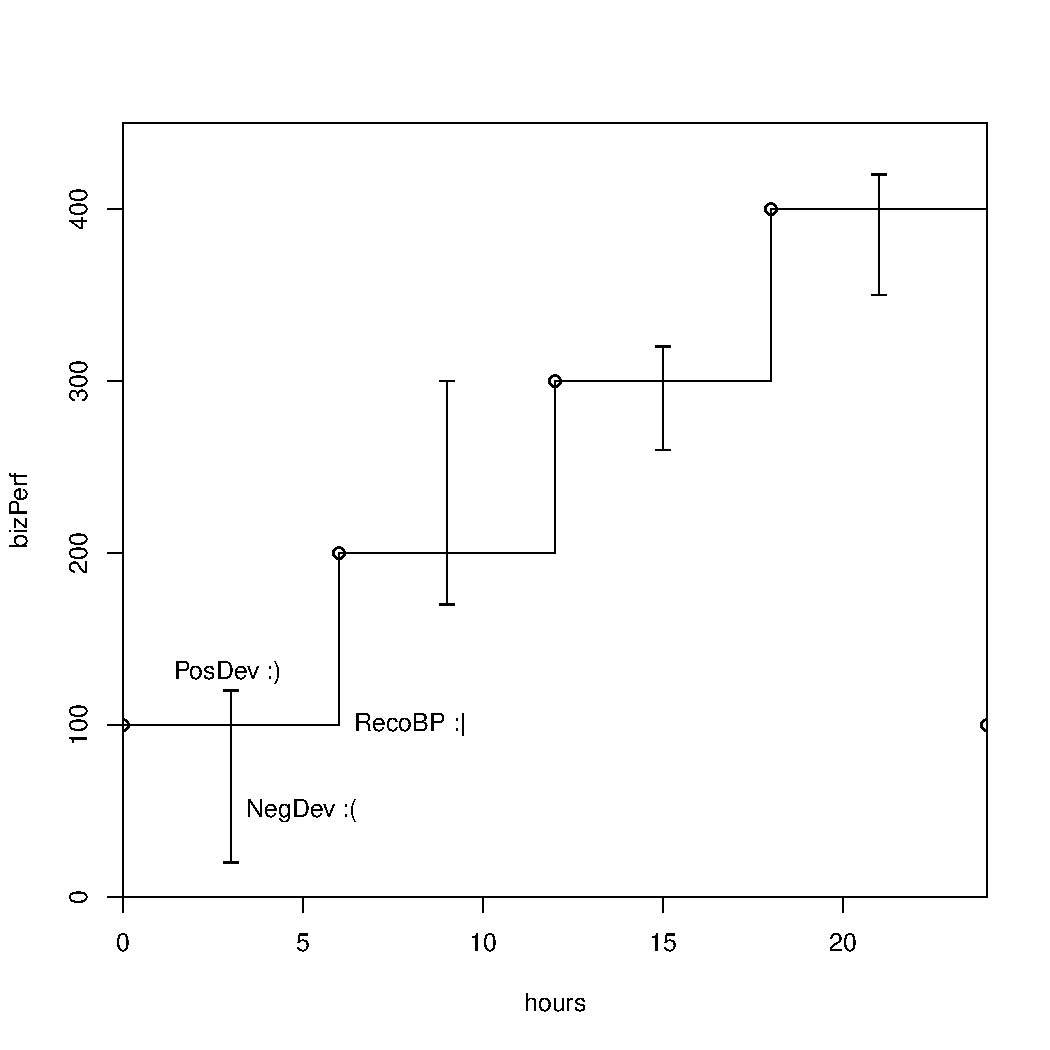
\includegraphics[width=0.99\linewidth]{generated/SFA-candles.pdf}
\caption{Software Flexibility Agreement representation}
\label{fig:EASC}
\end{figure}


The format of SFA is the following:

